\documentclass[12pt]{../manual}
%____________________________________________________________________________
%
%	TITLE AND TABLE OF CONTENTS
%____________________________________________________________________________
\begin{document}
\makeheader{Lab 3}
\begin{center}
\textbf{\huge ECE 230L - Lab 3 Pre-lab}\\~\\
\textbf{\large ALICE Windows Installation}\\~\\
\rule{6.5in}{0.5mm}\\
\end{center}

\tableofcontents

\newpage
%____________________________________________________________________________
%
%	BODY
%____________________________________________________________________________
\section{Windows 64 and 32 bit Installation Instructions}
\begin{enumerate}
\item Download the 64 Bit Libsmu software library installer package that contains the 64 Bit USB drivers for the ALM1000 \href{https://github.com/analogdevicesinc/libsmu/releases/download/v1.0.2/libsmu-1.0.2-setup-x64.exe}{here}. Download the link for the 32 bit libsmu library required to run ALICE1.3 for Windows  \href{https://github.com/analogdevicesinc/libsmu/releases/download/v1.0.2/libsmu-1.0.2-setup-x86.exe}{here}.
\item Now we will install the USB drivers. Run the libsmu-1.0.2-setup-x64.exe program you just downloaded for 64 bit Windows and run the libsmu-1.0.2-setup-x86.exe program you just downloaded for 32 bit Windows. Windows will warn you that the software is from an unknown publisher. Say Yes anyway. You will first be prompted to select a Setup Language.
\begin{figure}[!ht]
\begin{center}
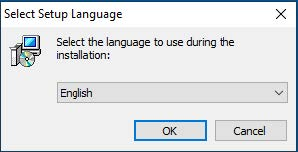
\includegraphics[width=0.5\textwidth]{figures/SetupLanguage}
\end{center}
\end{figure}
\item Accept the agreement below.
\begin{figure}[!ht]
\begin{center}
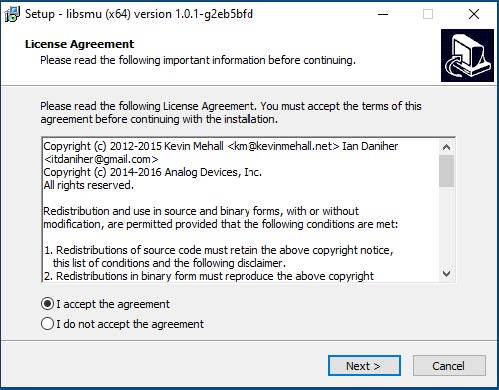
\includegraphics[width=0.5\textwidth]{figures/Agreement}
\end{center}
\end{figure}
\newpage
\item Next you will be asked to select a Destination Location. The default is fine. Click on Next.
\begin{figure}[!ht]
\begin{center}
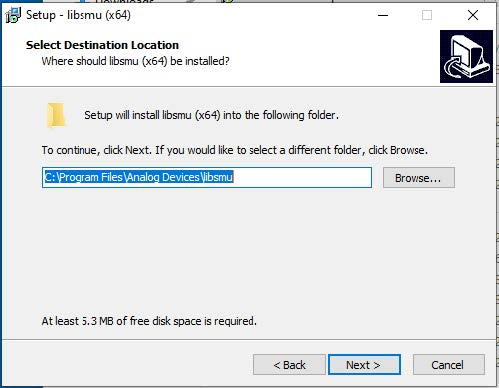
\includegraphics[width=0.5\textwidth]{figures/Destination}
\end{center}
\end{figure}
\item Next you will be asked to select what you want to install. By default just the install WinUSB drivers will be selected. That is all you will need.
\begin{figure}[!ht]
\begin{center}
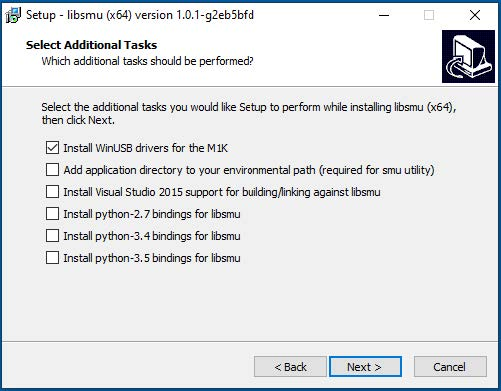
\includegraphics[width=0.5\textwidth]{figures/Installs}
\end{center}
\end{figure}
\newpage
\item The next thing to pop up is just to confirm that you wish to install the software. Click on Install.
\begin{figure}[!ht]
\begin{center}
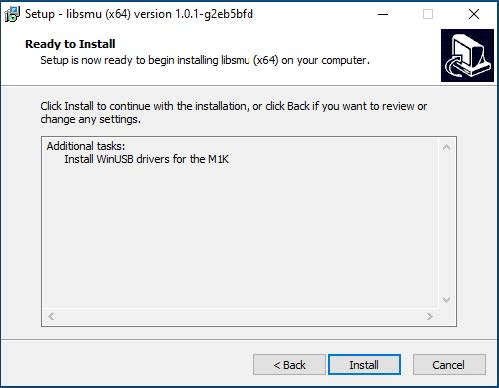
\includegraphics[width=0.5\textwidth]{figures/Installation}
\end{center}
\end{figure}
\item The Windows Driver install dialog box will now pop up. Click Next.
\begin{figure}[!ht]
\begin{center}
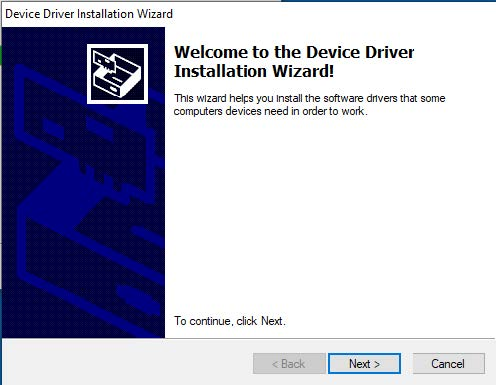
\includegraphics[width=0.5\textwidth]{figures/InstallationWizard}
\end{center}
\end{figure}
\newpage
\item If the USB driver Install completes you will get the last pop up screen:
\begin{figure}[!ht]
\begin{center}
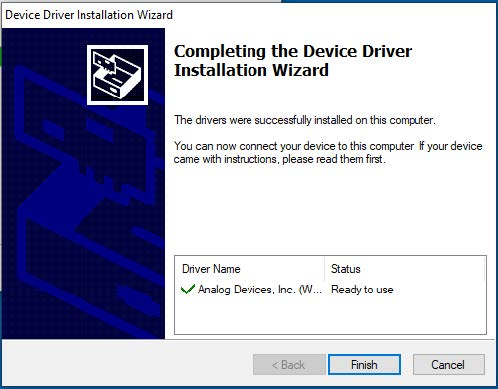
\includegraphics[width=0.5\textwidth]{figures/WizardDone}
\end{center}
\end{figure}
\item Click on Finish. The final pop-up should appear. Click on Finish.
\begin{figure}[!ht]
\begin{center}
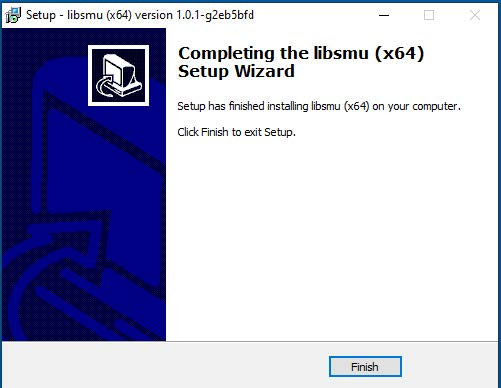
\includegraphics[width=0.5\textwidth]{figures/Finishing}
\end{center}
\end{figure}
\end{enumerate}

\newpage
\section{Windows 32 bit Installation Further Instructions}
\begin{enumerate}
\item Download the latest version of the Windows executable installer, alice-desktop-1.3-setup.exe, for ALICE 1.3 for the ALM1000  \href{https://github.com/analogdevicesinc/alice/releases}{here}. 
\item Next we will run the ALICE 1.3 Windows executable installer. Run the alice-desktop-1.3-setup.exe program you just down loaded. The first dialog to pop up asks you to select where you want to install the software. The default location is the best choice because the software writes certain files to the location where it runs so it needs to be somewhere that is not write protected. Click on Next.
\begin{figure}[!ht]
\begin{center}
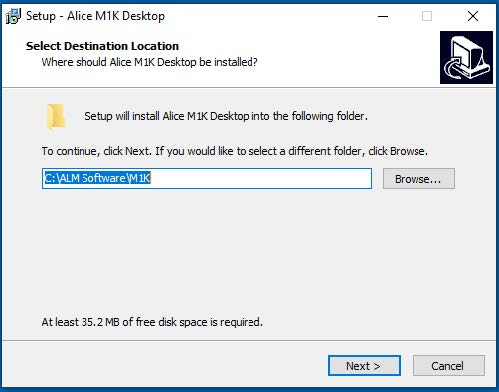
\includegraphics[width=0.5\textwidth]{figures/FileLoc}
\end{center}
\end{figure}
\item The next pop-up asks you to select the Start Menu Folder. The default location is fine. Click on Next.
\begin{figure}[!ht]
\begin{center}
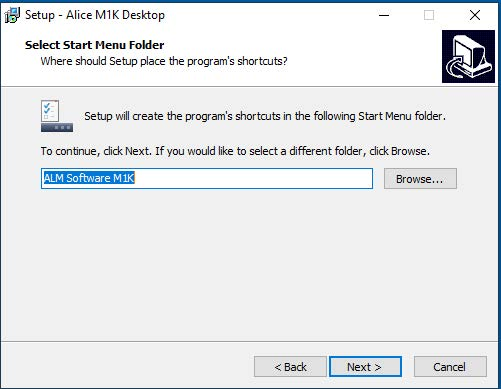
\includegraphics[width=0.5\textwidth]{figures/StartMenu}
\end{center}
\end{figure}
\newpage
\item The next pop-up just asks you to confirm that you want to install the software. Click on Next.
\begin{figure}[!ht]
\begin{center}
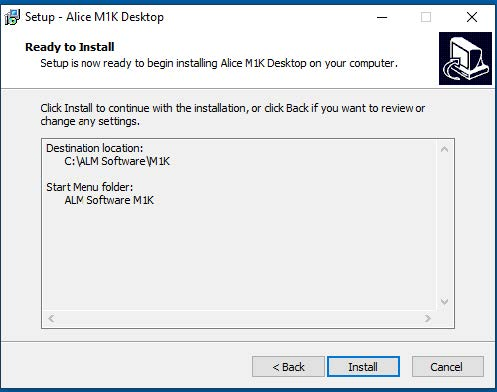
\includegraphics[width=0.5\textwidth]{figures/Confirm}
\end{center}
\end{figure}
\item When the installation completes this final dialog should appear. Click on Finish.
\begin{figure}[!ht]
\begin{center}
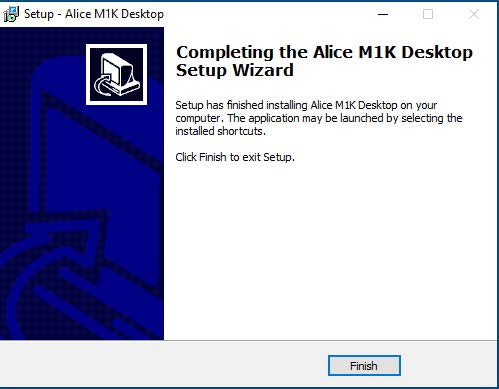
\includegraphics[width=0.5\textwidth]{figures/Done}
\end{center}
\end{figure}
\item After the software is installed a number of desktop icons should appear. You should now be able to plug-in your ADALM1000 to a USB port. Windows should recognize the new hardware and find the appropriate driver.
You are now ready to run ALICE 1.3. Start ALICE by double clicking on the desktop Icon.
\begin{figure}[!ht]
\begin{center}

\includegraphics[width=0.1\textwidth]{figures/DesktopIcon}
\end{center}
\end{figure}
\end{enumerate}

\newpage
\section{Troubleshooting}
\begin{enumerate}
\item Most likely your ADALM1000 has firmware version 2.16 installed from the factory (unless you used Pixelpulse2 to update the firmware already). ALICE will run with this version of the firmware but a couple of advanced capabilities of the hardware will not be available. Starting ALICE 1.3 with 2.16 firmware will give you the screen below at start-up. You can press OK to continue. 
\begin{figure}[!ht]
\begin{center}
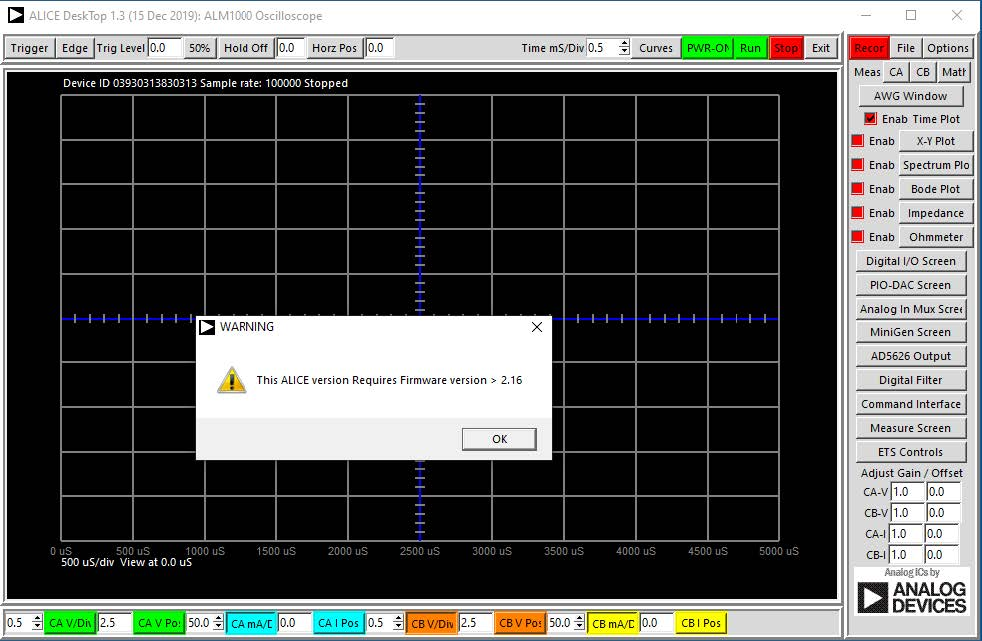
\includegraphics[width=0.5\textwidth]{figures/Troubleshooting1}
\end{center}
\end{figure}
\item This will happen each time ALICE starts until the new version 2.17 or higher of the firmware is flashed to the hardware. ALICE will then ask if you want to update the current firmware. Again you can skip this by saying No to use as is. This will happen each time ALICE starts until newer firmware is loaded. This firmware checking can be set to ignore by changing this line in the alice\_init.ini file:
global IgnoreFirmwareCheck; IgnoreFirmwareCheck = 0 \# change 0 to 1 to ignore firmware rev level.
\begin{figure}[!ht]
\begin{center}
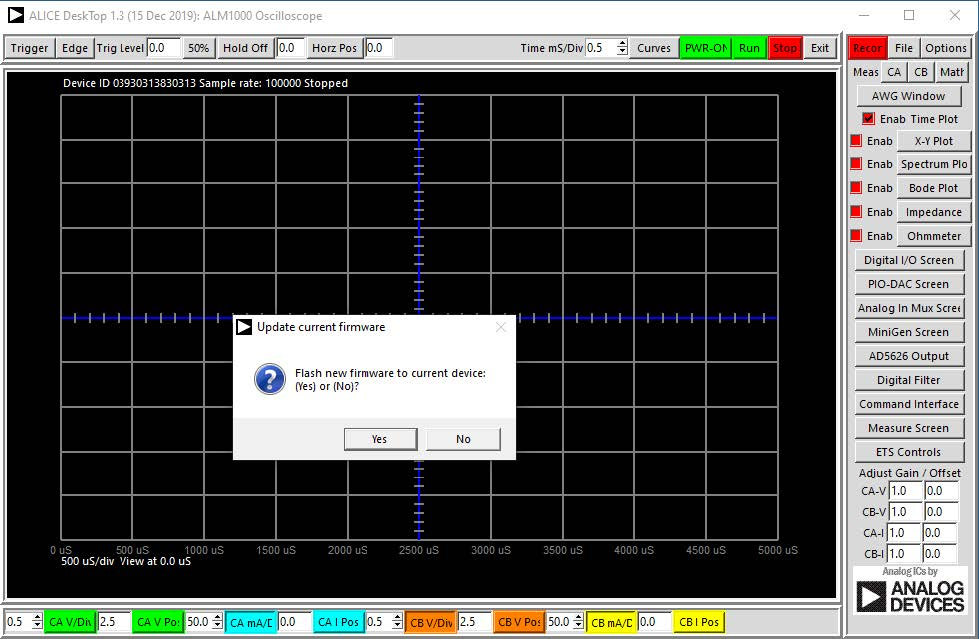
\includegraphics[width=0.5\textwidth]{figures/Troubleshooting2}
\end{center}
\end{figure}
\newpage
\item To update your board to the newest firmware click on the Options drop down menu. At the bottom of the list of options click on the Update Firmware button.
\begin{figure}[!ht]
\begin{center}
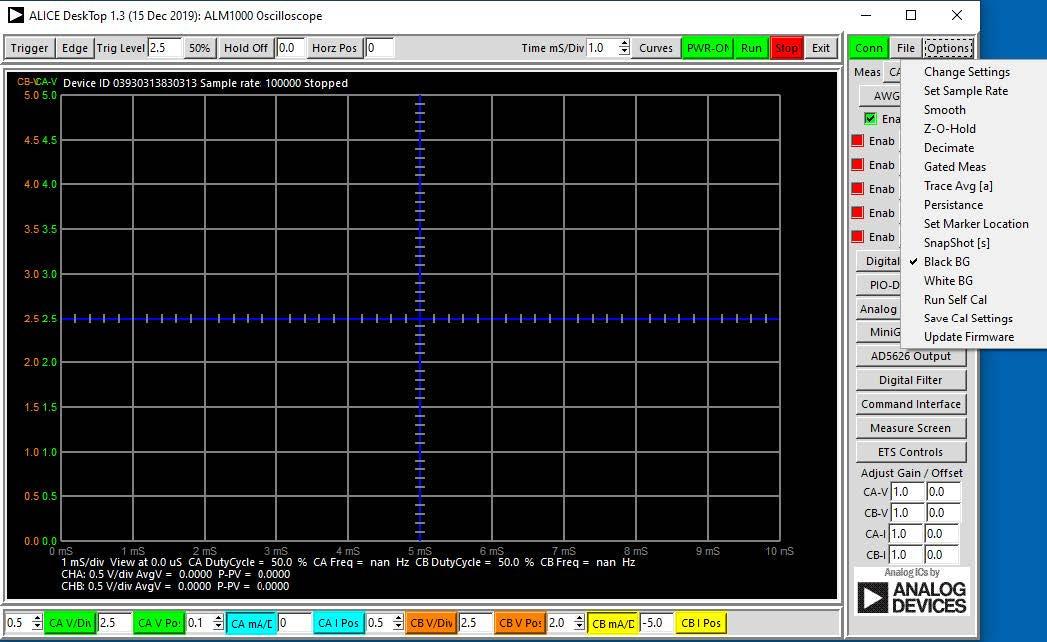
\includegraphics[width=0.5\textwidth]{figures/Troubleshooting3}
\end{center}
\end{figure}
\item The pop up dialog below will appear. Click on Yes.
\begin{figure}[!ht]
\begin{center}
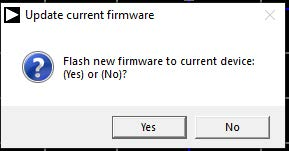
\includegraphics[width=0.5\textwidth]{figures/Troubleshooting4}
\end{center}
\end{figure}
\item A file selection dialog will appear. You may need to navigate to where the software was installed C:\textbackslash ALM Software\textbackslash M1K. Select the m1000-2.17.bin file and click on Open.
\begin{figure}[!ht]
\begin{center}
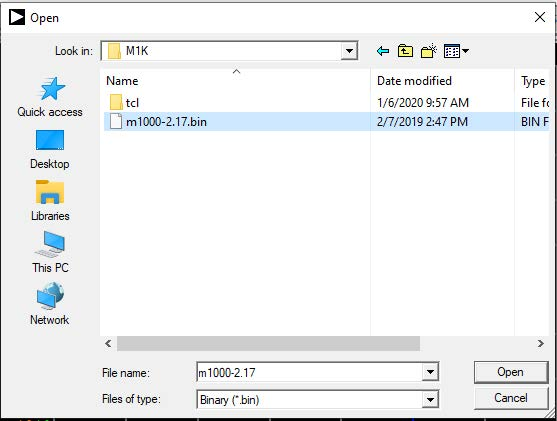
\includegraphics[width=0.5\textwidth]{figures/Troubleshooting5}
\end{center}
\end{figure}
\newpage
\item The program will pause for a few seconds while the board is being flashed. When it finishes the pop-up below should appear. Click on OK.
\begin{figure}[!ht]
\begin{center}
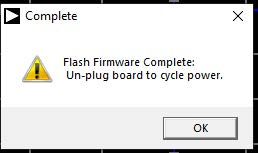
\includegraphics[width=0.3\textwidth]{figures/Troubleshooting6}
\end{center}
\end{figure}
\item You now need to unplug the board from the USB port to cycle the power. You also need to exit (close) ALICE. Click on OK and ALICE will close down.
\begin{figure}[!ht]
\begin{center}
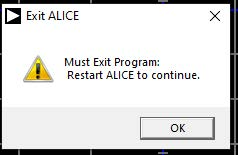
\includegraphics[width=0.3\textwidth]{figures/Troubleshooting7}
\end{center}
\end{figure}
\item Plug the ADALM1000 back into the USB port. Restart ALICE by double clicking on the desktop Icon. ALICE should start normally now. You can check the current state of the board firmware by clicking on the About button under the File drop down menu.
\begin{figure}[!ht]
\begin{center}
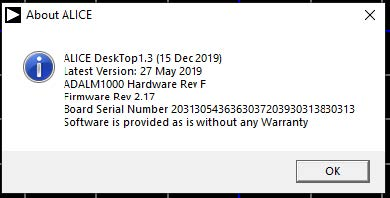
\includegraphics[width=0.3\textwidth]{figures/Troubleshooting8}
\end{center}
\end{figure}
\newpage
\item If for some reason the flashing of the firmware fails to happen properly you can try again by clicking on the Update Firmware button again. If all else fails you will either need to install Pixelpulse2 and flash the firmware with that program or go back and fully install the libsmu library that includes the smu command line utility (selecting the Add application directory to path variable option).
Using the Windows command prompt screen navigate to the directory where ALICE was installed C:\textbackslash ALM Software\textbackslash M1K and type smu. If the library was properly installed this should appear:
\begin{figure}[!ht]
\begin{center}
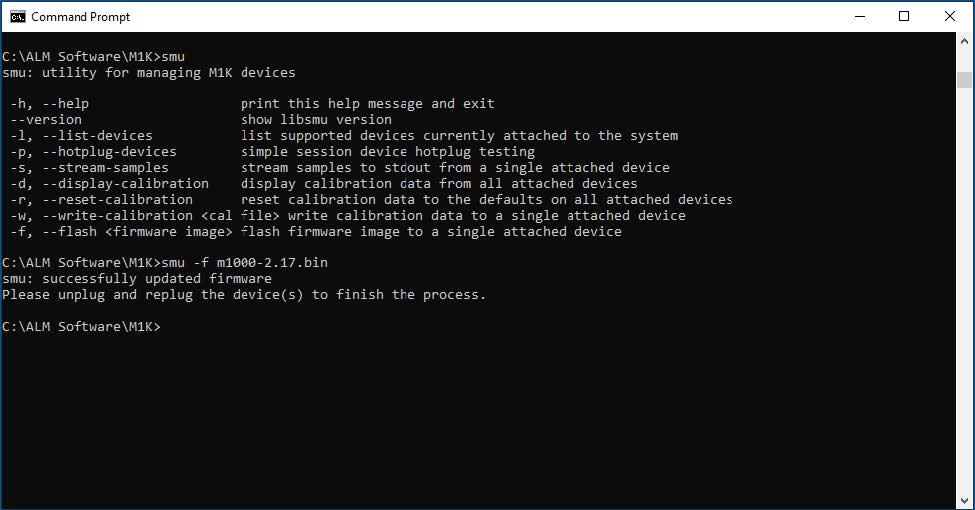
\includegraphics[width=0.7\textwidth]{figures/Troubleshooting9}
\end{center}
\end{figure}

Using the –f command line option for smu should flash the new firmware onto the board in all cases. You may need to cycle the power to the board before it can be recognized and in be in the right mode to be flashed.
\end{enumerate}
\end{document}
